\documentclass[a4paper]{article}
\usepackage{float}
\usepackage[english]{babel}
\usepackage[utf8]{inputenc}
\usepackage{amsmath}
\usepackage{graphicx}
\usepackage[colorinlistoftodos]{todonotes}
\usepackage{indentfirst}
\usepackage{courier}
\usepackage{subcaption}
\usepackage[section]{placeins}
\usepackage[
singlelinecheck=false 
]{caption}


\addtolength{\oddsidemargin}{-.875in}
\addtolength{\evensidemargin}{-.875in}
\addtolength{\textwidth}{1.75in}
\addtolength{\topmargin}{-.875in}
\addtolength{\textheight}{1.75in}

\title{Advanced Self-Organization Final Project\\Divison of Labor}

\author{Abbas Rizvi and Christine Anyansi\\VU University Amsterdam\\Amsterdam, Netherlands}

\date{\today}



\begin{document}
\maketitle

\newpage
\tableofcontents
\newpage

\begin{abstract}
Reinforced response threshold models are commonly used to  describe the self-organizing nature of ant colonies. Here we attempt to confirm and reproduce Gautrais' model. Additionally we attempt to discover the effect of changing a parameter from his model.  

%Past The model refers to the likelihood of an individual working on a task based off of its task-specific stimulus.   Individuals with low thresholds have a high probability to perform a task at a lower stimulus level than high threshold individuals.   When individuals work on a task, their internal threshold decreases and not working on a task increases their internal threshold.

Occurences of elitism, situations in which at least one working-elite develops, have been proven to appear in self-organizing ant colonies. Elitism in a society has not been well studied.  We were interested in the effect of reducing elitism and create a situation in which all individuals are contributing to the productivity to the colony.  Ultimately, we were able to reduce elitism by implementing a training function into Gautrais’ model.  Colonies shifted from having an elite work force to all individuals participating at some point through the simulation.
  
\end{abstract}

\section{Introduction}
Division of labor characterizes a self-organized system in which workers within a colony vary in the tasks they perform.  This concept can be applied to a variety of disciplines ranging from social insect societies to robotics to economics. Recent models have shown that social insect colonies act as self-organized, decentralized systems in which behavior emerges from the independent actions and decisions of workers.  Models of division labor must incorporate both variation in task performance among workers and individual worker flexibility \cite{Beshers}. By following a set of pre-defined behavioral rules, individuals can improve in productivity and performance by means of task repetition -- resulting in specialization towards a task.  %The concept of individual specialization demonstrates an underlying relationship as to how an entire colony behaves and the development of caste systems \cite{bonabeau}. 
Previous studies suggest that  specialization leads to the occurence of elitism in social insect colonies \cite{Gautrais}.  Elitism is defined as a situation when individuals tackle a disproportionately large portion of the work \cite{Gautrais}. The phenomenom of elitism, although observed in many research studies, has yet to be addressed on a practical level as a solvable problem \cite{Gautrais}\cite{evolution}\cite{bonabeau}.


%Response threshold models are well-established models that simulate division of labor. The idea behind response threshold models is simple -- they are designed such that individual workers have internal thresholds for responding to task-specific stimuli and worker will have a high probability of completing a task if the stimuli exceeds their own threshold \cite{bonabeau}.  Thresholds vary amongst individuals and those with the lowest thresholds will have preference to complete a task.  

Gautrais \textit{et al.}, 2002 used a reinforced response threshold model, an extension of a typical fixed response threshold model, to model division of labor in social insect colonies. The model was designed such that individual workers have internal thresholds for responding to task-specific stimuli and worker will have a high probability of completing a task if the stimuli exceeds their own threshold \cite{bonabeau}.  Thresholds vary amongst individuals and those with the lowest thresholds will have preference to complete a task. In Gautrais's original paper, he never specifies a max threshold for use in his model. Specifying a limit for each individual's threshold can have significant influence on a colony's overall work effort.



%A "learning" component was added to the individual workers such that the more often a worker confronts task $X$, it will reduce the worker's threshold for task $X$.  Therefore, the worker's probability to confront the same task again due to its lower stimulus has been reinforced.  Additionally, a "forgetting" concept was added to the model such that the thresholds for other tasks will increase over time, decreasing the probability for the worker to tackle the other task as a result of not encountering recently \cite{Gautrais}. 


In this study we have three main objectives. The first is to \textit{confirm}  the reinforced response threshold model detailed by Gautrais \cite{Gautrais}. Our second objective is to \textit{discover}  the influence of a max-threshold in the model. Lastly we aim to \textit{optimize} the model by introducing a "training" function. To further characterize these objectives five research questions were formulated with which to focus our research efforts.
\begin{enumerate}
  \item Under what conditions does elitism emerge?
  \item How do individuals specialize when there are two tasks to perform?
  \item What effect does limiting  individuals thresholds have on overall activity-level?
  \item How does a training option alter colony dynamics?
  \item What training options (if any) can reduce elitism in a colony?
\end{enumerate}


With these questions and objectives in mind, we formed our two hypotheses. We first hypothesize that implementation of a threshold is necessary in order to faithfully model self-organized ant colonies. Our second and main hypothesis is that a more "fair" society, in which all individuals contribute to the society, can be achieved by implementing a training option into the model. We continue to hypothesize that the earlier a training option is offered into a society, the more elitism can be reduced.   

This report is organized as follows. Section two introduces a brief summary of related past literature on this topic. Section three gives an overview of the model we base our experiments on. It is here that the theory behind the reinforced response threshold model is expounded upon. Section four provides the method in which we implemented our model. Here a pseudo-code with which we used to run our experiment is found. Section five goes on to state the our experimental procedure. It includes all variables that were tested, as well as the results and statistical analysis. Finally section six, the conclusion, offers a discussion of the results in which we answer the research questions and accept/reject our hypothesis. 



\section{Literature}
Response threshold models assume that individuals respond to a given task-specific stimulus when the stimulus exceeds the individual’s threshold can explain worker behavior flexibility at the colony level \cite{bonabeau}.  The more time that an individual spends working will decrease their own internal threshold coupled with decreasing the task-specific stimuli itself.   These models tend to result in elitism – a scenario in which only a portion the total population are constantly working and the remainder are not working \cite{Gautrais}\cite{evolution}\cite{bonabeau}. Several different versions of this model have been developed, which alter certain parameters, such as: colony size, variation on number of tasks (Gautrais \textit{et al.}, 2002) and genetic polymorphisms (Duarte \textit{et al.}, 2012) and their effects on the division of labor and overall colony performance.

The most relevant model (Gautrais \textit{et al.}, 2002) has two scenarios: (1) a group of individuals confronting a single task and (2) a group encountering two independent tasks.  Although the colony as a whole has more productivity, the individuals who are not engaging upon a task are not making any contributions to the production \cite{Gautrais}.   

This previous research does not consider elitism as a negative consequence.  It may not necessarily fair to the colony for some workers to be taking on the majority of work just because they are more fit to do so.  It is wasteful of total resources. We wanted to reduce elitism and observe if we could create society in which all individuals contribute to overall productivity. 

\section{Model}
The reinforced response threshold model (Gautrais \textit{et al.}, 2002) was used as a reference model in this study. The equations are designed such that an individual has a higher probability to initiate a response to a specific stimuli and begin working when the stimuli exceeds its own internal threshold.  The individual has a low (almost zero) probability to respond to a task stimulus if it's lower than the individual's threshold. Individuals may have different thresholds for different tasks. \cite{Gautrais}. 


\subsection{Task Stimulus-Level}
An individual may be engaged in only one task or in an idle latency period (not working).  When active, each individual works at the same, $\alpha$ units of work per time step.  Each task $T_j$ has a task-specific stimulus $S_j$ which increases by $\sigma_j$ per time step.  The stimulus is reduced by the number of individuals ($E_j$) working on the task multipied by their effort (work rate, $\alpha$). The value of one task stimulus is independent of the value of another task stimulus.  


The dynamics are described by:
\begin{equation}
dS_j = \sigma_j - E_j \times \alpha \;\; \forall = 1,2,\cdots,m
\end{equation}

\subsection{Stimulus Regeneration}


Stimulus regeneration, $\sigma_j$, a function of the colony capabilities, is characterized by:

\begin{equation}
\sigma_j = D \times W_{max}
\end{equation}

Where "demand" (\textit{D}) is a parameter (0 $<$ \textit{D} $\leq$ 1) defining the proportion of total effort the colony has to perform in order to complete the task. Such that \textit{D} = 1 refers to a colony working at maximum capacity. $W_{max}$ refers to the maximum amount of work a colony can perform at any given time:

\begin{equation}
W_{max} = \frac{N}{m}\frac{1}{1 + p}\alpha
\end{equation}


For $N$ individuals and $m$ tasks. \textit{p} is the probability that an individual will quit a task at random.



%To ensure that stimulus regeneration rate per capita was constant, a "demand" (0 $<$ \textit{D} $\leq$ 1) parameter was implemented such that it defined the amount of effort the total colony has to perform in order to complete the task.  \textit{D} = 1 refers to a colony working at maximum capacity. 

%\textit{D} $<$ 1 means that the dyanimcs of worker allocations will only fulfill minimum requirements to tackle the tasks.  Additionally, D represents the proportion of the colony that is working at that fixed period of time.  It allows comparisons between colonies of different sizes that are working a relative rate.  The absolute work rate when proportional to colony size is:



%The value of one task stimulus is independent of the value of another task stimulus. The small delay before workers begin to start working on a task is a result of the stimuli initialzation at 0 -- the stimuli are not large enough yet to stimulate the workers.


\subsection{Individuals}
For task $T_j$, each individual $i$ has a threshold $\theta_{i,j}$.  If the individual is idle, the individual may begin tackling a task if its internal threshold is less than the task-specific stimulus.  Each task has an equal probability of being tackled. Hence, when encountering a task $T_j$, the probability an individual $i$ tackles $T_j$ with an equal probability for $M$ tasks:

\begin{equation}
P(i\:engages\:in\:T_j) = \frac{1}{m} \frac{S_j^2}{S_j^2 + \theta_{i,j}^2}
\end{equation}

An actively working individual decreases the task-specific stimulus by $\alpha$.  A worker has the probability $p$ to randomly stop working. After an individual stops work, it experiences a latency period of one time step before it can work on a task again. An individual's threshold is initialized to zero.

\subsection{Learning and Forgetting}

An individual's internal threshold ($\theta$) for a specific task decreases every time step it works on the task. This is implemented into the model as a learning paramter $\xi$.  An individual's internal threshold increases every time step it does not work on that task. This is implemented as a forgetting parameter $\phi$. \\ 


Thus for individual $i$ engaged in task $j$:
\begin{subequations}
\begin{gather}
d\theta_{i,j} = - \xi \\
d\theta_{i,j\neq j'} = \phi \\
\theta_{i,j} = min(max(0,\theta_{i,j},\theta_j max) \; \forall i,j
\end{gather}
\end{subequations}


 
\subsection{Worker Specialization}

In order to describe dynamics of colonies with two tasks, a specialization variable (\textit{F}) is introduced. In this study it is presumed that an individual specializes when it prefers to continuously work on the same task. The variable, $C_i$, for individual $i$ refers to the proportion of total transitions that the individual has transitioned to a different task. For example: if an individual works on a series of tasks in this order: 1 1 2 1 1 2 - it transitioned to a different task three times within 5 transitions giving \textit{C} a value of 3/5 or 0.6. Thus  $F_i$, our metric of specialization,  varies from 0 (generalist workers) to 1 (full specialists) and is expressed by:

%amongst individuals, distinction between individuals who consistently work versus those that do not work often needs to be established.  To do this, activity level, which can be defined as the individual's $i$ time spent working during the simulation was measured.  The amount of "time" for the simulation was set to 20,000 time steps.  This proportion of time spent working also includes the period of differentation of individuals from the inital conditions ($i$,$j$ = 0 at time 0 $\forall$ $i$,$j$).  Typically after approximately 100 time steps,  individuals are well-differentiated and their thresholds are a good indicator of whether they are a generalist or a specialist \cite{Gautrais}.  


\begin{equation}
F_i = 1 - 2C_i
\end{equation}

Hence an individual consistantly works on the same task $F_i$ = 1, whereas an individual who randomly tackles tasks has $F_i$ = 0.

\subsection{Training}


One of the objectives of this study was to enhance the previous model by implementing a "training" option for individuals to partake in. This alternative was added with the expectation that training for individuals whose thresholds are past the point of no return would significantly reduce thresholds to a level capable of rejoining the working society. 

A variable, $\gamma$, was introduced to represent the amount of inactive time-steps before training would become available to inactive ants. After $\gamma$ time steps, an individual has a 50\% chance to undergo training for either task. Training, in the context of this model, refers to an 80\% reduction of the threshold. Additionally, the chance to work for the next time step is set to 100\% for when there is one task or 50\% for when there are two tasks.If an individual failed to undergo training, it became eligible to try again after $\gamma$ x .25 time steps. 




\section{Implementation}

Our simulations were implemented using NetLogo \cite{Netlogo}. The model was divided into time steps in which each individual’s own internal parameters were updated. The executables of each time step are detailed in the pseudo-code below. Each pseudo-code is followed by a text summarizing the stated code.\\ 


\noindent \textit{Global Parameters}\\
\texttt{Stimulus-regeneration ($\sigma$) set according to equation (2) \textit{\#this value is constant}\\
\noindent Calculate current stimulus-level:\\
\indent Stimulus-level task += stimulus-regeneration (($\sigma$) - (number-of-ants-working-on-task $\times$ work-per-step ($\alpha$))}\\

The above pseudo-code describes the method in which stimulus-level is calculated. The stimulus-regeneration value is the only globally constant parameter. The stimulus-level for each task is updated every time step according to the amount of ants working on the task and the pre-specified work done per task parameter.\\

\noindent \texttt{\textbf{for} every individual($i$), do this:\\
\indent \textbf{if} individual is already working on task $j$\\
\indent \indent  \#\textit{changes threshold value}\\
\indent \indent threshold ($\theta_{i,j}$) = maximum of 0 or (threshold ($\theta_{i,j}$) - learning ($\xi$))\\
\indent \indent threshold ($\theta_{i,k}$) = minimum of (threshold ($\theta_{i,k}$) + forgetting ($\phi$)) or max-threshold($T$)\\
\indent \indent \textit{\#k being the other task}\\
\indent\indent  \textbf{if} random float number from 0 to 1 < probability to quit($p$)\\
\indent \indent \textit{\#determines if worker will quit}\\
\indent \indent \indent working = 0}\\

The program checks each individual’s internal parameters every time step. If the individual’s working parameter is set to 1 (working on task 1) or 2 (working on task 2), the individual’s thresholds for each task are adjusted accordingly. The threshold of the task the individual is currently working on decreases by the pre-specified “learning” variable ($\xi$) while any other tasks thresholds increase by the “forgetting” variable ($\phi$). The ant then may possibly quit the task with a pre-specified probability ($p$). If the ant quits the task it’s internal working parameter will be set to 0.\\


\texttt{\textit{\#Calculates chance to work}\\
\indent \textbf{if} boredom $>$ max inactive steps($\gamma$)\\
\indent \textit{\#has chance to undergo training if idle for certain amount of time}\\
\indent \indent 50\% chance to undergo training \\
\indent \indent \textbf{if} undergoes training\\
\indent \indent \indent threshold ($\theta_{i,j}$) = threshold ($\theta_{i,j}$) $\times$ 0.80 \\
\indent \indent \indent chance-to-work = 1 / number of tasks ($m$)\\
\indent \indent \indent boredom = 0 \\
\indent \indent \textbf{elseif} two tasks, undergo same possibility of training for task 2\\
\indent \indent \textbf{else}\\
\indent \indent \indent boredom = boredom $\times$ 0.75\\ 
\indent \indent \textbf{else}\\
\indent \indent \indent chance-to-work on tasks set according to equation (4)}\\

The new training function implemented into our model comes into play here. If an ant has been inactive for longer than a pre-specified amount of time steps, the individual has a 50\% chance to undergo “training” for either task. Training, in the context of this model, simply results in an 80\% reduction of it’s threshold. It also sets the individual’s probability to work for the next turn to the max amount of certainty possible (100\% for one task, 50\% for two tasks). If the individual loses the 50/50 and does not undergo training, its counter for the amount of time steps inactive (“boredom”) will be set to 75\% of it’s current value, so that it can quickly have another chance to undergo training again. If the individual does not need training or if the training model is not activated the individual’s chance to work for each particular task is updated according to equation 2.\\

\texttt{\textbf{if} working = 0\\
\indent \indent boredom = boredom + 1\\
\indent \indent \textbf{for} both thresholds\\
\indent \indent \indent threshold($\theta_{i,j}$) = minimum of  ($\theta_{i,j}$ + $\phi$) and max-threshold ($T$)\\
\indent \indent \textbf{if} random number < chance-to-work on task\\
\indent \indent \indent working =  1 or 2\\
\indent \indent \indent \textit{\#depending on which task, 1 or 2, the ant will work during the next step}\\
\indent \indent \indent boredom = 0}\\

When the individual is not working (its working parameter is set to 0) it undergoes forgetting for both tasks. It then will determine whether it will work the next time step based on it’s internal chance-to-work parameter. If it will work, its “boredom” parameter is reset to 0. 



\section{Experiments}

\subsection{Design}

Our main goals were to 1) Confirm prior results, 2) investigate effect of adding a threshold and 3) investigate the effect of adding a training step. These main additions were tested on colonies of differing sizes, with differing demand levels, and differing number of tasks. Therefore, this study made use of the factorial experimental design. Dependent and independent variables used for Confirmation, Threshold, and Training experiments are detailed in Table 1 and Table 2, respectively.. \\



\begin{table}
\caption{Independent Variables}\label{table:1}
\begin{subtable}[t]{3in}
\centering
  \begin{tabular}{ | l | }
    \hline
     \textbf{Dependent Variables} \\ \hline
    Activity-Level \\ \hline
    Specialization-Level \\
    \hline
  \end{tabular}
  \caption{Confirmation and Threshold Experiment Variables}\label{table:1a}
 \end {subtable}
\quad
\begin{subtable}[t]{3in}
\centering
\begin{tabular}{ | l |}
    \hline
     \textbf{Dependent Variables}  \\ \hline
    Activity-Level \\ 
    \hline
  \end{tabular}
  \caption{Training Experiment Variables}\label{table:1b}
\end {subtable}
\end{table}

\begin{table}
\caption{Independent Variables}\label{table:2}
\begin{subtable}[H]{3in}
\centering
  \begin{tabular}{ | l | c | }
    \hline
     \textbf{Independent Variables} &  \textbf{Levels}  \\ \hline
    Colony Size ($N$) & 10, 100, 1000 \\ \hline
    Max-Threshold ($T$) & 1000, 10000000 \\
    \hline
    Number of Tasks ($m$) & 1,2\\ \hline
    Demand-Level ($D$) &	0.5, 0.8 \\ \hline
  \end{tabular}
  \caption{Confirmation and Threshold Experiment Variables}\label{table:2a}
 \end {subtable}
\quad
\begin{subtable}[H]{3in}
\centering
\begin{tabular}{ | l | c | }
    \hline
     \textbf{Independent Variables} &  \textbf{Levels}  \\ \hline
    Colony Size ($N$) & 10, 100, 1000 \\ 
    \hline
    Demand-Level ($D$) &	0.5, 0.8 \\ \hline
    Max-inactive ($\gamma$) & 40, 100 \\
    \hline
  \end{tabular}
  \caption{Training Experiment Variables}\label{table:2b}
\end {subtable}
\end{table}


\subsection{Setup}

Experiments were run on a 2012 model Linux. Each run consisted of 10,000 time-steps and every run was repeated 10 times. Table 3/4 contains the values of all other variables used in the Characterization, Threshold and Training experiments.


\begin{table}[H]
\caption{Other Variables}\label{table:3}
\begin{subtable}[H]{3in}
\centering
  \begin{tabular}{ | l | c | }
    \hline
     \textbf{Other Variables} &  \textbf{Levels}  \\ \hline
    Starting Stimulus level ($\theta$) & 0\\ \hline
    Work-per-step ($\alpha$) & 0.1 \\
    \hline
    Probability to quit task ($p$) & 0.2\\ \hline
    Learning ($\xi$) &	4 \\ \hline
    Forgetting ($\phi$) & 10 (1 task), 3.5 (2 tasks) \\ \hline
  \end{tabular}
  \caption{Confirmation and Threshold Experiment Variables}\label{table:3a}
 \end {subtable}
\quad
\begin{subtable}[H]{3in}
\centering
\begin{tabular}{ | l | c | }
    \hline
     \textbf{Other Variables} &  \textbf{Levels}  \\ \hline
    Starting Stimulus Level ($\theta$) & 0\\  \hline
     Work-per-step ($\alpha$) & 0.1 \\
    \hline
    Probability to quit task ($p$) & 0.2\\ \hline
    Learning ($\xi$) &	4 \\ \hline
    Forgetting ($\phi$) & 10  \\ \hline
    Number of Tasks ($m$) & 1 \\ \hline
    Max-Threshold ($T$) & 1000 \\ \hline
  \end{tabular}
  \caption{Training Experiment Variables}\label{table:3b}
\end {subtable}
\end{table}
\FloatBarrier

\subsection {Results}


\subsubsection {Threshold}


This study first aimed to reproduce the results made by Gautrais in his original model (2002). Gautrais never implicitly mentioned having a threshold in his model, however this must have been the case as shown in Figure 1, only when a threshold is implemented were we able to reproduce the self organizing model stated by Gautrais. Runs in which thresholds were set very high, activity levels were limited to the two extremes - working the max amount of time or never working.

\begin{figure}[!ht]
	\begin{subfigure}[b]{0.45\linewidth}
      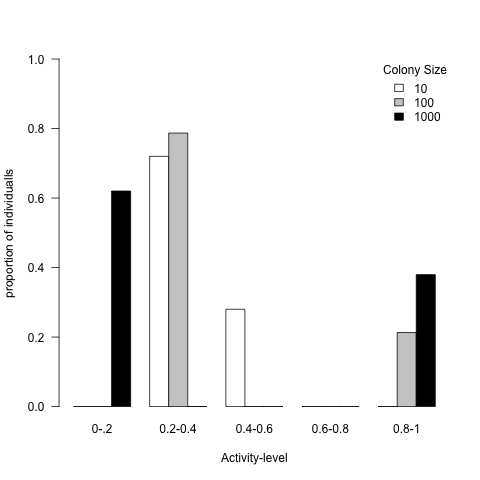
\includegraphics[width=\linewidth]{Threshold_1_task_and_5_demand_with_1000T}
		\caption{Threshold 1000}\label{fig:1a}		
	\end{subfigure}
    \hfill
    \begin{subfigure}[b]{0.45\linewidth}
      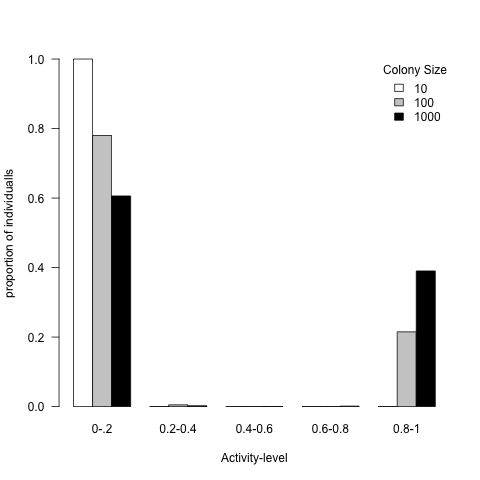
\includegraphics[width=\linewidth]{Threshold_1_task_and_5_demand_and_1000000T}
		\caption{Threshold 10000000}\label{fig:1b}
	\end{subfigure}
	\caption{Differing activity levels among ant colonies of increasing size for two different max-threshold values, 1000 (a), or 10000000 (b). For both sets of runs, $D$ = 0.5, $m$ = 1 (1 task), $\alpha$ = 0.1, $\xi$ = 4, and $\phi$ = 10.  See section 5.1 and 5.2 for further parameter information.}\label{fig:1}
\end{figure}



\subsubsection {Two Tasks}

To further confirm Gaustrais’ model, simulations were done for situations in which there are two tasks. With more than one tasks, individuals have the chance to preferentially choose one over the other – to \textit{specialize}. The equation for each individual’s specialization level is stated in 3.5. Figure 2 shows how the application of a threshold effects specialization and activity level. Here we replicate the finding that specialization increases with increasing colony size and demand. Additionally, when compared to the activity-levels observed in Figure 1, a decrease in the max activity-level is observed when there are two tasks (~0.83 with one task, 0.72~ with two tasks). This can be explained by the decreased chance to engage in a task when there are more options as seen in equation 2, the probability to engage in a task is limited by 1/m. m being the number of tasks. 

\begin{figure}[!ht]
    \begin{subfigure}[b]{0.45\linewidth}
      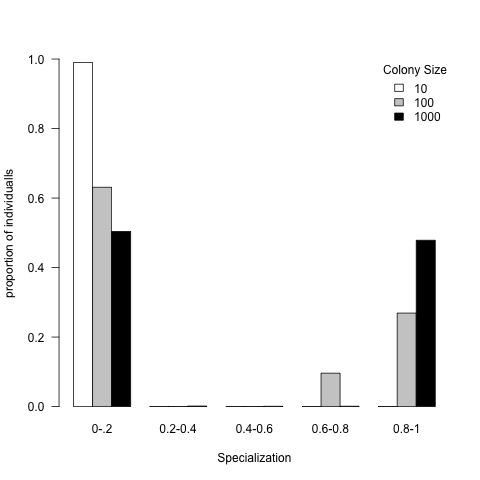
\includegraphics[width=\linewidth]{2_Tasks_Spe_Demand_5}
      \caption{Specialization - Demand 0.5}\label{fig:2a}
    \end{subfigure}
    \hfill
    \begin{subfigure}[b]{0.45\linewidth}
      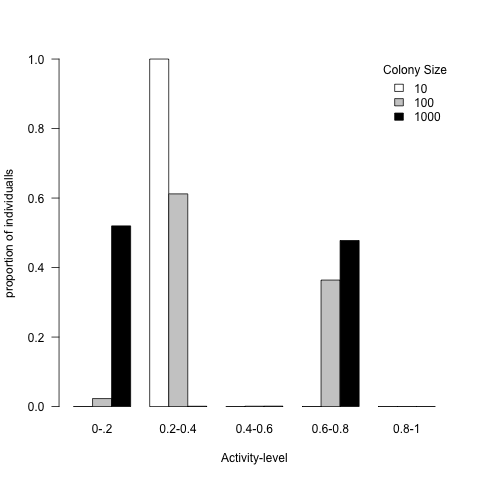
\includegraphics[width=\linewidth]{2_Tasks_Act1_demand_5}
      \caption{Activity-Level - Demand 0.5}\label{fig:2c}
     \end{subfigure}
     
     \begin{subfigure}[b]{0.45\linewidth}
      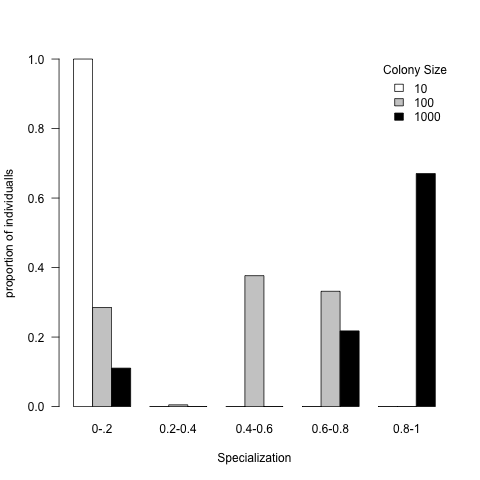
\includegraphics[width=\linewidth]{2_Tasks_Spe_and_8_demand}
      \caption{Specialization - Demand 0.8}\label{fig:2b}
    \end{subfigure}
    \hfill
    \begin{subfigure}[b]{0.45\linewidth}
      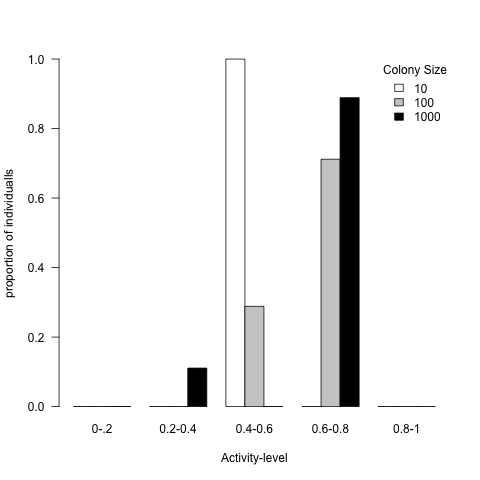
\includegraphics[width=\linewidth]{2_Tasks_Act_and_8_demand}
      \caption{Activity-Level - Demand 0.8}\label{fig:2d}
     \end{subfigure}
     \caption{Specialization levels of colonies with $D$ = 0.5 (a) and $D$ = 0.8 (c) and Activity levels of colonies with $D$ = 0.5 (b) and $D$ = .8 (d). In all cases, $m$ = 2 (2 tasks), $\alpha$ = 0.1, $\xi$ = 4, and $\phi$ = 3.5.  See section 5.1 and 5.2 for further parameter information.}\label{fig:2}


\end{figure}


\subsubsection {Training}

In order to answer the problem of elitism, the model was optimized with the addition of a training function. Figure 3 shows the effect of a training option to ant colonies of $m$ = 1 (1 task) and differing demand levels.  The specifics of the training function can be found in Section 4. An individual has an option to undergo training after either 40 or 100 inactive steps. Results suggest that elitism can be effectively reduced when training is possible after 40 steps for ants of all colony sizes.   


\begin{figure}[!ht]
    \begin{subfigure}[b]{0.45\linewidth}
      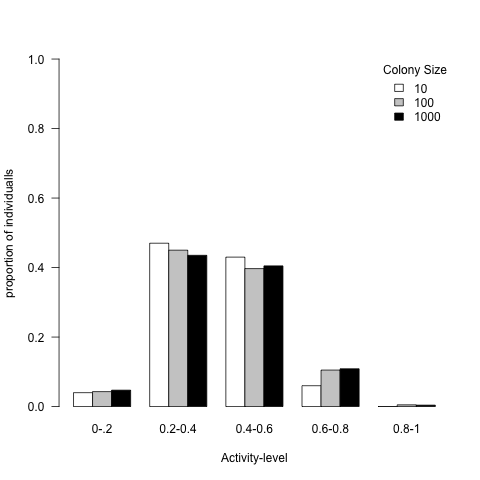
\includegraphics[width=\linewidth]{Boredom_40_and_5}
      \caption{$\gamma$ = 40 - Demand 0.5}\label{fig:3a}
    \end{subfigure}
    \hfill
    \begin{subfigure}[b]{0.45\linewidth}
      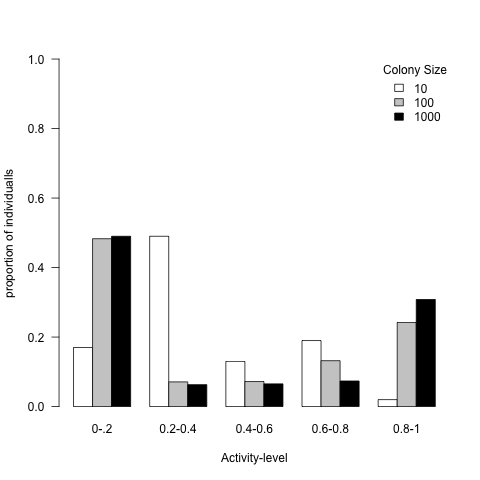
\includegraphics[width=\linewidth]{Boredom_100_and_5}
      \caption{$\gamma$ = 100 - Demand 0.5}\label{fig:3b}
     \end{subfigure}
     
     \begin{subfigure}[b]{0.45\linewidth}
      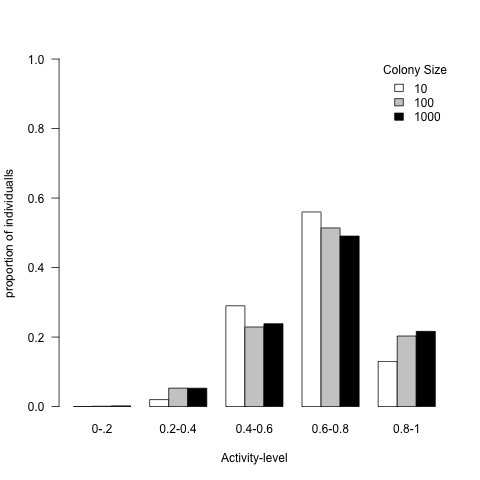
\includegraphics[width=\linewidth]{Boredom_40_and_8}
      \caption{$\gamma$ = 40 - Demand 0.8}\label{fig:3c}
    \end{subfigure}
    \hfill
    \begin{subfigure}[b]{0.45\linewidth}
      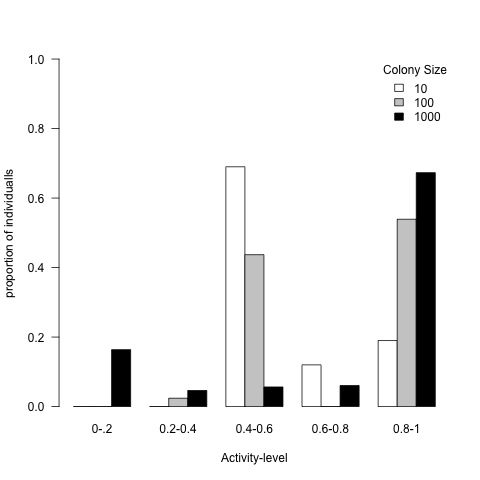
\includegraphics[width=\linewidth]{Boredom_100_and_8}
      \caption{$\gamma$ = 40 - Demand 0.5}\label{fig:3d}
     \end{subfigure}
     \caption{Differing activity-levels for ant colonies with a training option enacted after 40 (a and c) and 100 (b and d) time steps with $D$ = 0.5 and $D$ = 0.8 In all cases, $m$ = 1 (1 task), $\alpha$ = 0.1, $\xi$ = 4, and $\phi$ = 3.5.  See section 5.1 and 5.2 for further parameter information.}\label{fig:3}


\end{figure}





\subsection{Output Analysis}
\begin{table}[H]
\caption{Comparison of activity level between different size colonies with the same overall demand, implementing a maximum threshold.}\label{table:4}
\begin{tabular}{|l|l|l|l|l|}
\hline
\textbf{Colony Size}   & 100         & 100            & 1000         & 1000            \\ \hline
\textbf{Demand ($D$)}        & 0.5         & 0.5            & 0.5          & 0.5             \\ \hline
\textbf{Max Threshold ($\gamma$)} & 1000        & 10000000       & 1000         & 10000000        \\ \hline
                       & \multicolumn{2}{l|}{p = 0.8} & \multicolumn{2}{l|}{p = 0.008} \\ \hline
\end{tabular}
\end{table}



As mentioned in 5.3.1, Gautrais \textit{et al.}, 2002 did not explicitly mention implementing a maximum threshold.  Data was analyzed by Welch’s t-test to compare when a threshold of 1000 was set against a very high threshold that a stimulus would most likely never reach.   The t-test was only run for groups of 100 and 1000 as a very small colony of 10 does not have any activity level at the upper extreme (0.8 – 1) activity level (Figure 1a, 1b).  A colony size of 100 accepts the null hypothesis (p = 0.8).  A colony size of 1000 shows a strong presumption against the null hypothesis (p = 0.008).  


\begin{table}[H]
\caption{Comparison between activity level of increasing demand from 0.5 to 0.8 and increasing colony size.}
\label{table:5}
\begin{tabular}{|l|l|l|l|l|l|l|}
\hline
\textbf{Colony Size} & 10                 & 10                & 100                & 100               & 1000               & 1000              \\ \hline
\textbf{Demand ($D$)}      & 0.5                & 0.8               & 0.5                & 0.8               & 0.5                & 08                \\ \hline
                     & \multicolumn{2}{l|}{p \textless 0.001} & \multicolumn{2}{l|}{p \textless 0.001} & \multicolumn{2}{l|}{p \textless 0.001} \\ \hline
\end{tabular}
\end{table}

As discussed in 5.3.2 – validation of Gautrais et al., 2002’s model – a comparison was conducted using Welch’s t-test was used to compare to determine if there were significant changes in activity-level when demand level was increased.  The null hypothesis was rejected for all changes in colony size (Table 5).

\begin{table}[H]
\caption{Comparison of activity level between different colony sizes of trained and untrained groups with same demand.}
\begin{tabular}{|l|l|l|l|l|}
\hline
                           & \textbf{Trained}  & \textbf{Untrained} & \textbf{Trained}  & \textbf{Untrained} \\ \hline
\textbf{Colony Size}       & 100               & 100                & 1000              & 1000               \\ \hline
\textbf{Demand ($D$)}            & 0.5               & 0.5                & 0.5               & 0.5                \\ \hline
\textbf{Max Threshold ($T$)}     & 1000              & 1000               & 1000              & 1000               \\ \hline
\textbf{Max Time Inactive ($\gamma$)} & 40                & 10000000           & 40                & 10000000           \\ \hline
                           & \multicolumn{2}{l|}{p \textless 0.001} & \multicolumn{2}{l|}{p \textless 0.001} \\ \hline
\end{tabular}
\end{table}

In order to observe the effect of training, we used Welch’s t-test to compare no training (max time inactive = 10000000) against training (max time inactive = 40).  Only the extremes (0.8-1.0) activity level was used in this test, as we wanted to observe if there was a reduction in the amount of individuals doing all of the work.  The null hypotheses were rejected for colony sizes of 100 and 1000. 


\begin{table}[H]
\caption{Comparison of activity level between trained groups with the same demand but differences in max time inactive.}
\begin{tabular}{|l|l|l|l|l|l|l|}
\hline
                           & \textbf{Trained}   & \textbf{Trained}  & \textbf{Trained}   & \textbf{Trained}  & \textbf{Trained}   & \textbf{Trained}  \\ \hline
\textbf{Colony Size}       & 100                & 100               & 1000               & 1000              & 1000               & 1000              \\ \hline
\textbf{Demand ($D$)}            & 0.5                & 0.5               & 0.5                & 0.5               & 0.5                & 0.5               \\ \hline
\textbf{Max Time Inactive ($\gamma$)} & 40                 & 100               & 40                 & 100               & 40                 & 100               \\ \hline
                           & \multicolumn{2}{l|}{p \textless 0.001} & \multicolumn{2}{l|}{p \textless 0.001} & \multicolumn{2}{l|}{p \textless 0.001} \\ \hline
\end{tabular}
\end{table}

Welch’s t-test was conducted on different colony sizes with the same demand, comparing if there was a difference from a maximum of 40 time steps and 100 times steps (Figure 3).  Colony size of 10 accepts the null hypothesis.  Colony sizes of 100 and 1000 reject the null hypothesis (Table 7).  

\section{Conclusion}

\subsection{Confirmation of Reference Model}

Our first objective was to confirm the findings from Gautrais’ reinforced response threshold model \cite{Gautrais}.  We reproduced their model using NetLogo \cite{Netlogo}.  Gautrais original model was designed such that individual workers have internal thresholds for responding to task-specific stimuli.  A worker has a high probability to complete a task if the stimulus exceeds the worker’s individual threshold.  His model also suggested that with increasing colony size there would be more elitism – that is a disproportional amount of individuals work while many other individuals do not work.\\  

\noindent\textit{Under what conditions does elitism emerge?}\\
\indent Elitism develops by means of when an individual working on a specific task – he is able to lower his own threshold for that task and has preference to work on the task again.  This makes it less likely for individuals who have not worked on the task previously to work on it in the future and those who have worked on a task before will continue to work.\\  

\noindent\textit{What effect does limiting individuals' thresholds have on overall activity-level?}\\
\indent When we reproduced Gautris model using the same equations and parameter settings – we were not able to obtain the same results (Figure 1a). Referring to other literature, we deduced that there must have been an implementation of a maximum threshold in order to ensure that the individual threshold levels were not forever increasing \cite{evolution}.

Our second objective was to \textit{discover} the influence of a maximum threshold on the model.  We implemented this by running simulations with a maximum threshold of 1000 and a maximum threshold of 1000000 (high enough for a task-stimulus to not reach without being worked on first by workers with lower thresholds).  Figure 1b shows that when a maximum threshold is applied, the results appear to validate Gautrais’ model.   Statistics were run on the data produced from the simulations to compare the differences of colony size and maximum threshold (Table 4).  Colony sizes of 100 (p = 0.8) do not show statistical significance that by implementing maximum threshold that the occurrence of elitism is increased.  Conversely, colony sizes of 1000 (p = 0.008) provide a strong presumption that there will be increased instances of elitism when a maximum threshold is applied to the model (Table 4).  Therefore, we presume that Gautrais must have implemented a maximum threshold in his model in order to obtain his results published in Gautrais et al., 2002, confirming our first hypothesis. \\   

\noindent\textit{How do individual specialize when there are two tasks to perform?}\\
\indent We confirmed Gautrais’ hypothesis that when an additional task was added to the simulation, specialization increases on a task as colony size increases.  We compared activity-level with specialization at a constant demand of 0.5. Activity-levels for colonies of 100 showed that approximately 40\% of the individuals were working 60-80\% of the time and approximately 60\% were working 20-40\% of the time (Figure 2b).  Also, a colony size of 100 had 25\% of individuals’ specialization at the upper extreme (0.8 – 1.0) and 60\% at the lower extreme (0.0 – 0.2, Figure 2a). A colony size of 1000 showed that approximately 50\% of the population was actively working 60-80\% of the time and 50\% of the population was only working approximately 0-20\% of the time (Figure 2b). A colony size of 1000 also showed increased specialization when compared to a colony size of 100 (Figure 2a).  An increase in demand from 0.5 to 0.8, both increased specialization and activity-level for all colony sizes (Figure 2c, 2d).  These findings confirm Gautrais’ hypothesis that with increased colony size, there is increased specialization.


\subsection{Optimization of Model}
The previous findings show that overall activity-level increases with increased colony size, but with the consequence of elitism.  This is not fair to the colony as a whole because a disproportional amount of individuals are not making any contribution to the system.  We hypothesized that we may be able to achieve a colony that had a fairly distributed working force, essentially reducing elitism by implementing a training function.\\  


\noindent\textit{How does a training option alter colony dynamics?}\\
\indent Response threshold for individuals to task-specific stimuli continuously increase when an individual is not working.  We can prevent a worker’s threshold from increasing to the point where there is virtually a zero probability that the worker will ever have a task-stimulus exceed his own threshold by implementation of a training function.  The mathematical design behind the training function can be found in section 3.6.\\

\noindent\textit{What training options (if any) can reduce elitism in a colony?}\\
\indent We ran statistics on the differences between colonies that had no training (max inactive time = 10000000) against those who are trained (max inactive time = 100).  Colony size of 100 and 1000 both had p $<$ 0.001, indicating that statistical significant amount of the population for both colony sizes are no longer working all the time – and that the work must be becoming more evenly distributed amongst all individuals (Table 6).  Thus confirming our hypothesis that a training parameter will distribute the amount of work conducted on a task more evenly throughout an entire colony

We wanted to optimize the training function.  We examined max inactivity times of 40 and 100 across all colony sizes.  Comparing figure 3a and 3b – a lower max time step of 40 shows a greater number of individuals working at all colony levels with the same demand level ($D$ = 0.5).  When the demand is increased it appears that entire population is at least working at some point for all colonies (Figure 3c, 3d).  It is statistically significant (p $<$ 0.001, Table 7) that less individuals are 80-100\% active for all time steps for colony sizes of 100 and 1000. 

\subsection{Discussion}
In conclusion, we successfully reproduced Gautrais \textit{et al.}, 2002 reinforced response threshold model.  We confirmed his findings by finding a suitable maximum threshold for the model. The model showed that workers would tend towards elitism. We were able to reduce elitism by introducing a training function into the model. In this paper we clearly show that individuals in an ant colony do exhibit self-organizing tendencies. Each have their own internal model that drives them to behave independently of each other. The individuals of an ant colony are able to sponatneously organize their members to achieve the goal of completing a task. This property of ant colonies is has been characterized and implemented in this study.

There are many additonal questions regarding the behavior of this model that were not included here.  In the Gaustrais \textit{et al.}, 2002 paper -- for two tasks they only looked at specialization and not activity-level. Activity-level of a colony where there are two tasks would provide more insite into the worker dynamics. In cases where specialization is low, it is important to differentiate whether it is low due to lack of overall work effort, or simply due to lack of specializing. It would also be prudent to investigate the effect high demand levels ($>$ 0.8) have on specialization of a colony. 





\pagebreak
\begin{thebibliography}{9}

\bibitem{Gautrais}
Gautrais, Jacques, et al. "Emergent polyethism as a consequence of increased colony size in insect societies." Journal of Theoretical Biology 215.3 (2002): 363-373.
\bibitem{Beshers}
Beshers, Samuel N., and Jennifer H. Fewell. "Models of division of labor in social insects." Annual review of entomology 46.1 (2001): 413-440.
\bibitem{Netlogo}
Wilensky, U. (1999). NetLogo. http://ccl.northwestern.edu/netlogo/. Center for Connected Learning and Computer-Based Modeling, Northwestern University, Evanston, IL
\bibitem{evolution}
Duarte, Ana, et al. "Evolution of self-organized division of labor in a response threshold model." Behavioral ecology and sociobiology 66.6 (2012): 947-957.
\bibitem{bonabeau}
Theraulaz, Guy, Eric Bonabeau, and J. N. Denuebourg. "Response threshold reinforcements and division of labour in insect societies." Proceedings of the Royal Society of London. Series B: Biological Sciences 265.1393 (1998): 327-332.

\end{thebibliography}

\clearpage


\end{document}